% Sustentación del Taller 4 (lógica difusa; tema Beamer institucional UD). Compilar:  make slides
% Las cifras (\cifra...) salen de ../informe/numeros.tex, generado por desarrollo/exportar_informe.py.
\documentclass[aspectratio=169,10pt]{beamer}
\usepackage[spanish,es-noshorthands]{babel}
\usetheme{UD}
% Generado por desarrollo/exportar_informe.py: NO editar a mano.
\newcommand{\cifrapropMamdani}{5,5586}
\newcommand{\cifrapropSugeno}{5,3445}
\newcommand{\cifrapropIrisReglas}{16}
\newcommand{\cifrapropIrisAcc}{0,889}
\newcommand{\cifrapropIrisAri}{0,729}
\newcommand{\cifratodoUnoA}{flavanoids}
\newcommand{\cifratodoUnoB}{proline}
\newcommand{\cifratodoUnoC}{OD280/OD315}
\newcommand{\cifratodoUnoD}{alcohol}
\newcommand{\cifratodoUnoFA}{188}
\newcommand{\cifratodoUnoFB}{149}
\newcommand{\cifratodoUnoFC}{127}
\newcommand{\cifratodoUnoFD}{100}
\newcommand{\cifrapropCurvaReglas}{0,2: 66, 0,3: 15, 0,4: 8, 0,5: 4, 0,6: 4, 0,7: 3, 0,8: 3, 0,9: 3, 1,0: 3}
\newcommand{\cifrapropRidgeSin}{45,1\,\%}
\newcommand{\cifrapropCvTresRidge}{90,3\,\%}
\newcommand{\cifrapropTestTresRidge}{96,3\,\%}
\newcommand{\cifrapropPureza}{0,927}
\newcommand{\cifrapropAri}{0,794}
\newcommand{\cifrapropFpc}{0,690}
\newcommand{\cifrapropFrontera}{20}
\newcommand{\cifrapropPurezaKm}{0,927}
\newcommand{\cifrapropMalAgrupados}{13}
\newcommand{\cifrapropRMejor}{0,8}
\newcommand{\cifrapropReglasMejor}{3}
\newcommand{\cifrapropAccMejor}{94,4\,\%}
\newcommand{\cifrapropCvUno}{45,1\,\%}
\newcommand{\cifrapropCvDos}{95,2\,\%}
\newcommand{\cifrapropCvTres}{96,0\,\%}
\newcommand{\cifratuneEntAntes}{0,145}
\newcommand{\cifratuneEntDesp}{0,095}
\newcommand{\cifratuneValAntes}{0,260}
\newcommand{\cifratuneValDesp}{0,254}
\newcommand{\cifratuneEntSin}{0,0006}
\newcommand{\cifratuneValSin}{0,384}
\newcommand{\cifratuneIter}{1}
\newcommand{\cifratuneIters}{40}
\newcommand{\cifratuneAccAntes}{90,7\,\%}
\newcommand{\cifratuneAccDesp}{94,4\,\%}
\newcommand{\cifratuneValSubida}{47}
\newcommand{\cifraveinteWMdos}{0,806 $\pm$ 0,049}
\newcommand{\cifraveinteReglasWMdos}{9,7 $\pm$ 1,2}
\newcommand{\cifraveinteWMtres}{0,865 $\pm$ 0,047}
\newcommand{\cifraveinteReglasWMtres}{24,1 $\pm$ 3,4}
\newcommand{\cifraveinteWMcuatro}{0,931 $\pm$ 0,036}
\newcommand{\cifraveinteReglasWMcuatro}{41,9 $\pm$ 2,9}
\newcommand{\cifraveinteSubTres}{0,881 $\pm$ 0,078}
\newcommand{\cifraveinteReglasSubTres}{14,8 $\pm$ 2,8}
\newcommand{\cifraveinteSubCinco}{0,956 $\pm$ 0,024}
\newcommand{\cifraveinteReglasSubCinco}{5,0 $\pm$ 0,9}
\newcommand{\cifraveinteSubOcho}{0,946 $\pm$ 0,024}
\newcommand{\cifraveinteReglasSubOcho}{3,0 $\pm$ 0,0}
\newcommand{\cifraveinteArbol}{0,894 $\pm$ 0,044}
\newcommand{\cifrapropSelDistintas}{2}
\newcommand{\cifrapropPermMax}{95,6\,\%}
\newcommand{\cifrapropPermMin}{90,4\,\%}
\newcommand{\cifrapropPermWM}{86,5\,\%}
\newcommand{\cifraadicN}{5456}
\newcommand{\cifraadicTrain}{3856}
\newcommand{\cifraadicTest}{1600}
\newcommand{\cifraadicDupCuatro}{50}
\newcommand{\cifraadicDupDos}{279}
\newcommand{\cifraadicRacha}{6,5}
\newcommand{\cifraadicCambios}{395}
\newcommand{\cifraadicSharp}{2097}
\newcommand{\cifraadicSlightR}{826}
\newcommand{\cifraadicForward}{2205}
\newcommand{\cifraadicSlightL}{328}
\newcommand{\cifraadicDosReglas}{6}
\newcommand{\cifraadicDosW}{0,02}
\newcommand{\cifraadicDosAcc}{99,81}
\newcommand{\cifraadicDosBal}{99,88}
\newcommand{\cifraadicDosF}{99,88}
\newcommand{\cifraadicDosMF}{2\,$\times$\,3}
\newcommand{\cifraadicCuatroReglas}{24}
\newcommand{\cifraadicCuatroW}{0,02}
\newcommand{\cifraadicCuatroAcc}{99,50}
\newcommand{\cifraadicCuatroBal}{99,39}
\newcommand{\cifraadicCuatroF}{99,45}
\newcommand{\cifraadicCuatroMF}{2\,$\times$\,3\,$\times$\,2\,$\times$\,2}
\newcommand{\cifraadicCorteFrente}{0,9005}
\newcommand{\cifraadicCorteIzqA}{0,4945}
\newcommand{\cifraadicCorteIzqB}{0,9015}
\newcommand{\cifraadicAutoDosMin}{91,4\,\%}
\newcommand{\cifraadicAutoDosMax}{96,1\,\%}
\newcommand{\cifraadicAutoCuatroMin}{78,7\,\%}
\newcommand{\cifraadicAutoCuatroMax}{95,2\,\%}
\newcommand{\cifraadicAutoReglasMin}{48}
\newcommand{\cifraadicAutoReglasMax}{100}
\newcommand{\cifraadicKnnBloques}{85,6\,\%}
\newcommand{\cifraadicKnnMuestra}{94,0\,\%}
\newcommand{\cifraadicKnnInfla}{8,3}
\newcommand{\cifraadicMamdaniDosCero}{97,8\,\%}
\newcommand{\cifraadicMamdaniDosGrande}{58,2\,\%}
\newcommand{\cifraadicGanadoraDosGrande}{92,6\,\%}


\newcommand{\pts}{\,pts}
\newcommand{\cifraGrande}[3]{\begin{minipage}[t]{0.3\linewidth}\centering
  {\cambriafont\fontsize{14pt}{16pt}\selectfont\bfseries\color{#3}#1\par}{\fontsize{7pt}{8.5pt}\selectfont\color{UDSilver}#2\par}\end{minipage}}
\newcommand{\txt}[1]{{\fontsize{7.3pt}{9pt}\selectfont #1\par}}

\begin{document}

\UDportada{Lógica difusa: reglas desde datos y modelos para un robot}
          {Taller 4: propuesto (Wine) y adicional (robot)}
          {Juan Felipe Rodríguez Galindo\\{\fontsize{6.4pt}{7.4pt}\selectfont\mdseries\color{UDSilver}20261595004}}
          {Maestría en Ciencias de la Información y las Comunicaciones}
          {Inteligencia Computacional Aplicada}

%% ------------------------------------------------------------------ 2
\begin{frame}{Qué se pidió y qué se hizo}{Dos entregas con la misma fecha: Taller Propuesto (punto 3) y Taller Adicional (punto 4)}
  \begin{columns}[T,onlytextwidth]
    \begin{column}{0.48\textwidth}
      \UDCard{white}{UDBorder}{\cardtitle{UDBlue}{Punto 3 · Taller Propuesto}{\fontsize{7.5pt}{9.2pt}\selectfont
        Revisar el script resuelto del profesor (Mamdani, Sugeno, Wang--Mendel, FCM) y repetir su flujo con \textbf{Wine}: TODO 1 a 5 y el ejemplo \textit{Tune FIS}. Hecho en Python.\par}}
    \end{column}
    \begin{column}{0.48\textwidth}
      \UDCard{UDLightGray}{UDRed!60}{\cardtitle{UDRed}{Punto 4 · Taller Adicional}{\fontsize{7.5pt}{9.2pt}\selectfont
        Dos modelos difusos (4 y 2 sensores) para clasificar el movimiento de un robot, con las MF salidas del análisis de datos y máximo 100 reglas.\par}}
    \end{column}
  \end{columns}
  \vspace{0.35cm}
  \begin{center}
  \begin{tikzpicture}[node distance=0.28cm]
    \node[paso] (a) {\textbf{Revisar}\\script del profesor};
    \node[paso, right=of a] (b) {\textbf{Reproducir}\\9 referencias};
    \node[paso, right=of b] (c) {\textbf{Wine}\\TODO 1 a 5};
    \node[paso, right=of c, fill=UDRed!8, draw=UDRed] (d) {\textbf{Robot}\\6 y 24 reglas};
    \draw[flecha] (a) -- (b); \draw[flecha] (b) -- (c); \draw[flecha] (c) -- (d);
  \end{tikzpicture}
  \end{center}
\end{frame}

%% ------------------------------------------------------------------ 3
\begin{frame}{El script del profesor: qué hace y qué supone}{Se reprodujeron sus 9 valores de referencia con código propio}
  \begin{columns}[T,onlytextwidth]
    \begin{column}{0.50\textwidth}
      \UDCard{white}{UDBorder}{\cardtitle{UDBlue}{Lo que recorre}{\fontsize{7.2pt}{8.8pt}\selectfont
        \textbf{MF y operadores} $\to$ \textbf{Mamdani} (propina \cifrapropMamdani) $\to$ \textbf{Sugeno 0} (\cifrapropSugeno) $\to$ \textbf{Wang--Mendel} en \textit{Iris} (\cifrapropIrisReglas{} reglas, \cifrapropIrisAcc) $\to$ \textbf{FCM} (ARI \cifrapropIrisAri) $\to$ reglas frente a un árbol.\par}}
    \end{column}
    \begin{column}{0.46\textwidth}
      \UDCard{UDLightGray}{UDRed!60}{\cardtitle{UDRed}{Supuestos que no se dicen}{\fontsize{7.2pt}{8.8pt}\selectfont
        \textbf{1.} La salida del Sugeno se redondea a un número de clase: supone clases \textbf{ordenadas}.\\
        \textbf{2.} Si ninguna regla se activa, la clase por defecto es 0.\\
        \textbf{3.} Todo sale de \textbf{una} partición pequeña (45 pruebas en \textit{Iris}).\par}}
    \end{column}
  \end{columns}
  \vspace{0.3cm}
  \txt{Estos tres puntos guiaron el desarrollo propio: se midió el efecto de la numeración de clases, se evitó confiar en una sola partición (20 particiones) y se usó validación para elegir parámetros.}
\end{frame}

%% ------------------------------------------------------------------ 4
\begin{frame}{Wine: TODO 1 y TODO 2}{Selección de 4 características con ANOVA y reglas de Wang--Mendel}
  \begin{columns}[T,onlytextwidth]
    \begin{column}{0.46\textwidth}
      \UDCard{white}{UDBorder}{\cardtitle{UDBlue}{TODO 1 · ANOVA (solo entrenamiento)}{\fontsize{7.2pt}{8.8pt}\selectfont
        \cifratodoUnoA{} (F = \cifratodoUnoFA), \cifratodoUnoB{} (\cifratodoUnoFB), \cifratodoUnoC{} (\cifratodoUnoFC), \cifratodoUnoD{} (\cifratodoUnoFD). En 20 particiones, solo \cifrapropSelDistintas{} conjuntos distintos: la selección es estable.\par}}
    \end{column}
    \begin{column}{0.50\textwidth}
      \UDCard{UDLightGray}{UDGold}{\cardtitle{UDGold}{TODO 2 · reglas desde datos}{\fontsize{7.2pt}{8.8pt}\selectfont
        \resizebox{\linewidth}{!}{\begin{tabular}{lrrrr}
\toprule
Etiquetas $n$ & Reglas & Rejilla $n^4$ & Exactitud prueba & Árbol (mismas hojas) \\
\midrule
2 & 10 & 16 & 75,9\,\% & 87,0\,\% \\
3 & 31 & 81 & 92,6\,\% & 87,0\,\% \\
4 & 43 & 256 & 88,9\,\% & 87,0\,\% \\
\bottomrule
\end{tabular}
}\par}}
    \end{column}
  \end{columns}
  \vspace{0.2cm}
  \txt{Las reglas son el 62\,\%, 38\,\% y 17\,\% de la rejilla $n^4$: salen solo de las combinaciones que existen. En esta partición $n=3$ supera a $n=4$, pero con 54 vinos de prueba un acierto vale 1,85 puntos: es ruido (en 20 particiones el orden es monótono).}
\end{frame}

%% ------------------------------------------------------------------ 5
\begin{frame}{TODO 3: agrupamiento sustractivo}{Menos reglas al subir r, y un sobreajuste que una sola partición no muestra}
  \begin{columns}[T,onlytextwidth]
    \begin{column}{0.50\textwidth}
      \UDCard{white}{UDBorder}{\cardtitle{UDBlue}{Reglas y exactitud}{\fontsize{7pt}{8.6pt}\selectfont
        \resizebox{\linewidth}{!}{\begin{tabular}{lrrrr}
\toprule
Radio $r$ & Reglas & Exact. entren. & Exact. prueba & NaN en prueba \\
\midrule
0,3 & 15 & 99,2\,\% & 90,7\,\% & 0 \\
0,5 & 4 & 96,8\,\% & 94,4\,\% & 0 \\
0,8 & 3 & 96,0\,\% & 94,4\,\% & 0 \\
\bottomrule
\end{tabular}
}\par}}
      \vspace{0.1cm}
      \txt{Con $r\ge0{,}7$ quedan 3 reglas, una por cultivar.}
    \end{column}
    \begin{column}{0.46\textwidth}
      \UDCard{UDLightGray}{UDRed!60}{\cardtitle{UDRed}{El fallo de r = 0,3}{\fontsize{7.2pt}{8.8pt}\selectfont
        15 reglas $\times$ 5 coeficientes $\approx$ 75 parámetros para 124 vinos. En validación cruzada: \cifrapropRidgeSin{} y salidas de hasta $2\cdot10^{6}$. Con \textit{ridge} 0,1: \cifrapropCvTresRidge.\par}}
    \end{column}
  \end{columns}
\end{frame}

%% ------------------------------------------------------------------ 6
\begin{frame}{TODO 4 y TODO 5}{Fuzzy C-Means y el equivalente de la app Fuzzy Logic Designer}
  \begin{columns}[T,onlytextwidth]
    \begin{column}{0.46\textwidth}
      \UDCard{white}{UDBorder}{\cardtitle{UDBlue}{FCM sin etiquetas}{\fontsize{7.2pt}{8.8pt}\selectfont
        Pureza \cifrapropPureza, ARI \cifrapropAri; k-means da la misma pureza. Lo que aporta lo difuso: \cifrapropFrontera{} de 178 vinos tienen grado máximo $<0{,}6$ (frontera).\par}}
      \vspace{0.12cm}
      \UDCard{UDLightGray}{UDGold}{\cardtitle{UDGold}{Mejor sistema (validación cruzada)}{\fontsize{7.2pt}{8.8pt}\selectfont
        $r=\cifrapropRMejor$: \cifrapropReglasMejor{} reglas, exactitud en prueba \cifrapropAccMejor. R2 (todo alto $\to$ clase 1) es la más fácil de leer.\par}}
    \end{column}
    \begin{column}{0.50\textwidth}
      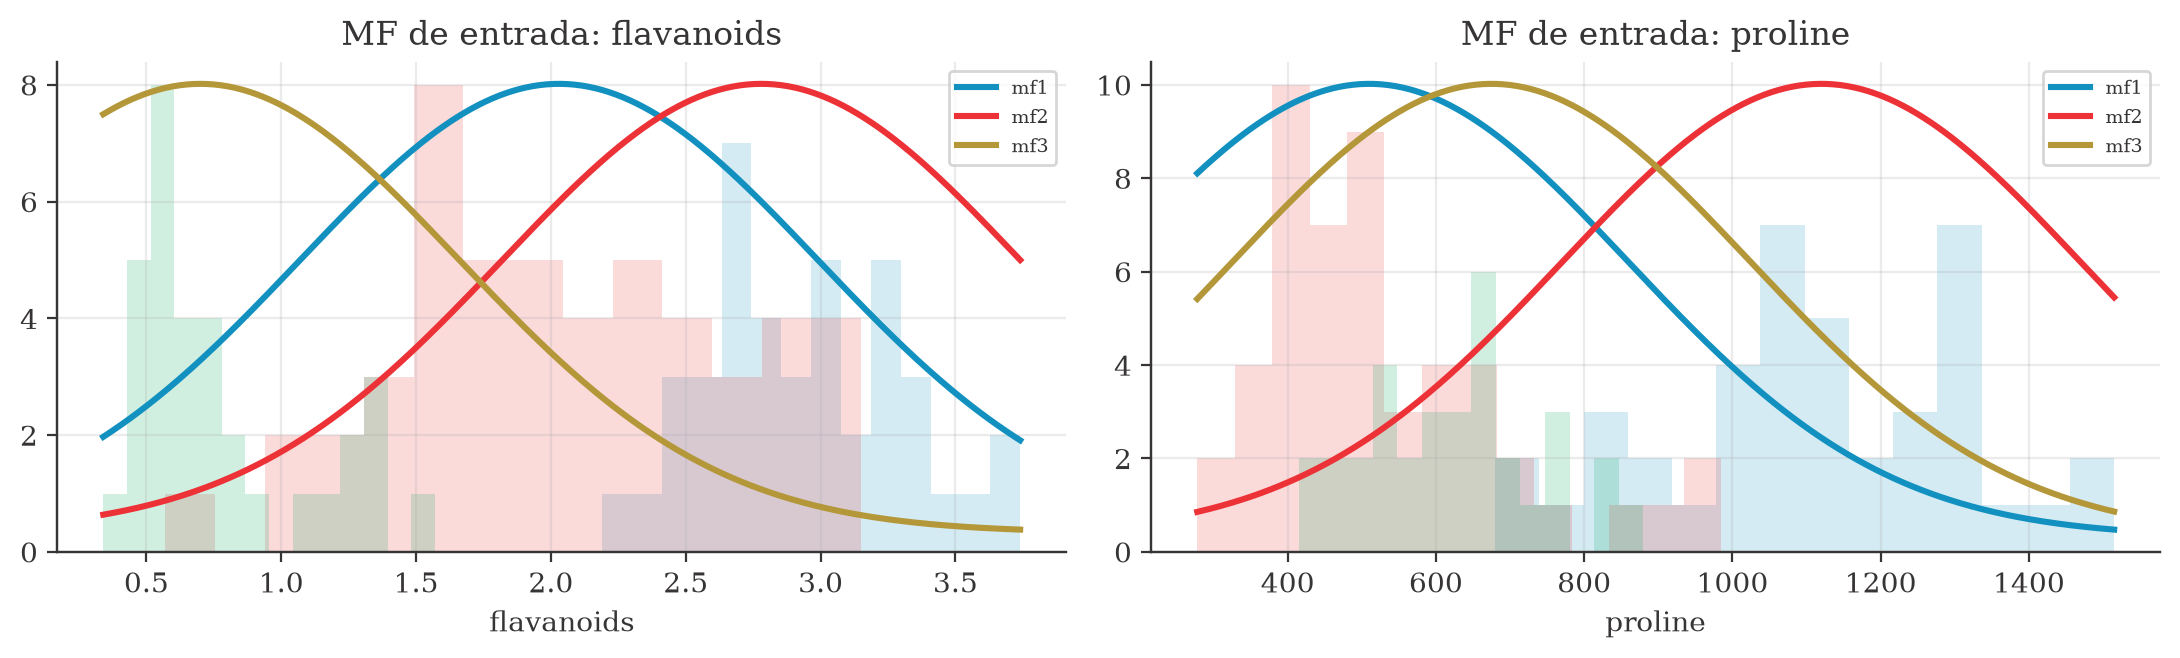
\includegraphics[width=\linewidth]{figuras/prop_f04_mf_entrada.png}\par\vspace{0.1cm}
      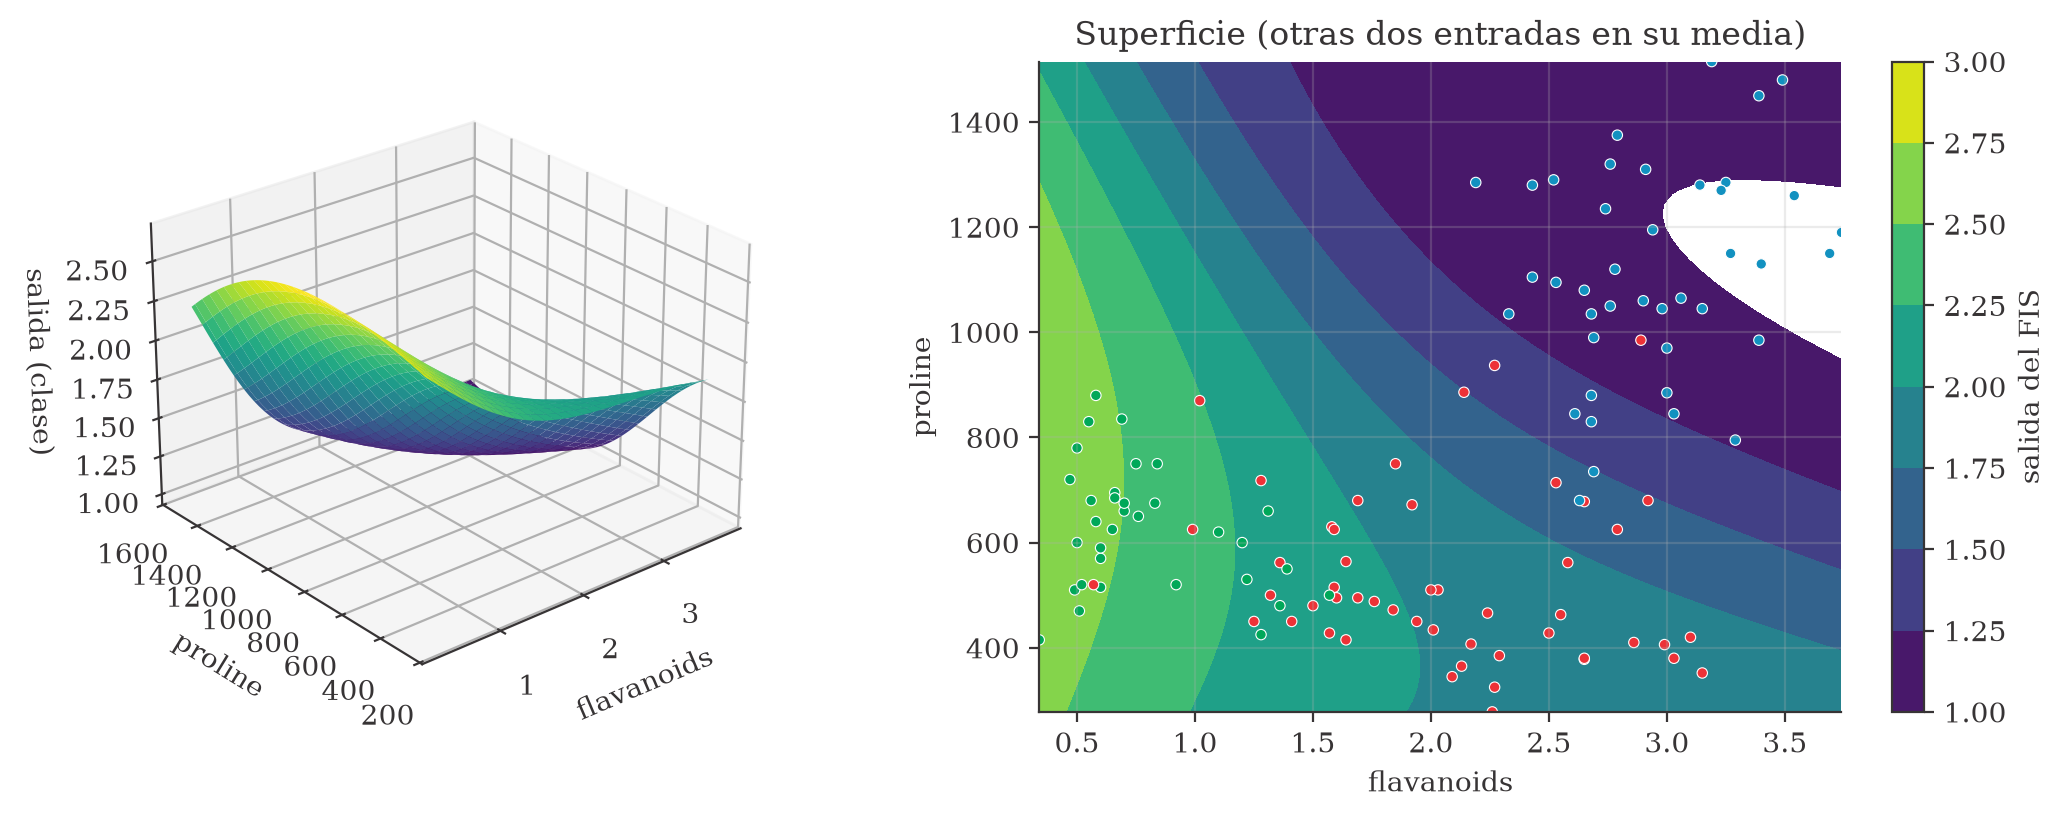
\includegraphics[width=0.85\linewidth]{figuras/prop_f05_superficie.png}
    \end{column}
  \end{columns}
\end{frame}

%% ------------------------------------------------------------------ 7
\begin{frame}{Extra: Tune FIS y numeración de clases}{Dos advertencias sobre procedimientos que parecen inocentes}
  \begin{columns}[T,onlytextwidth]
    \begin{column}{0.58\textwidth}
      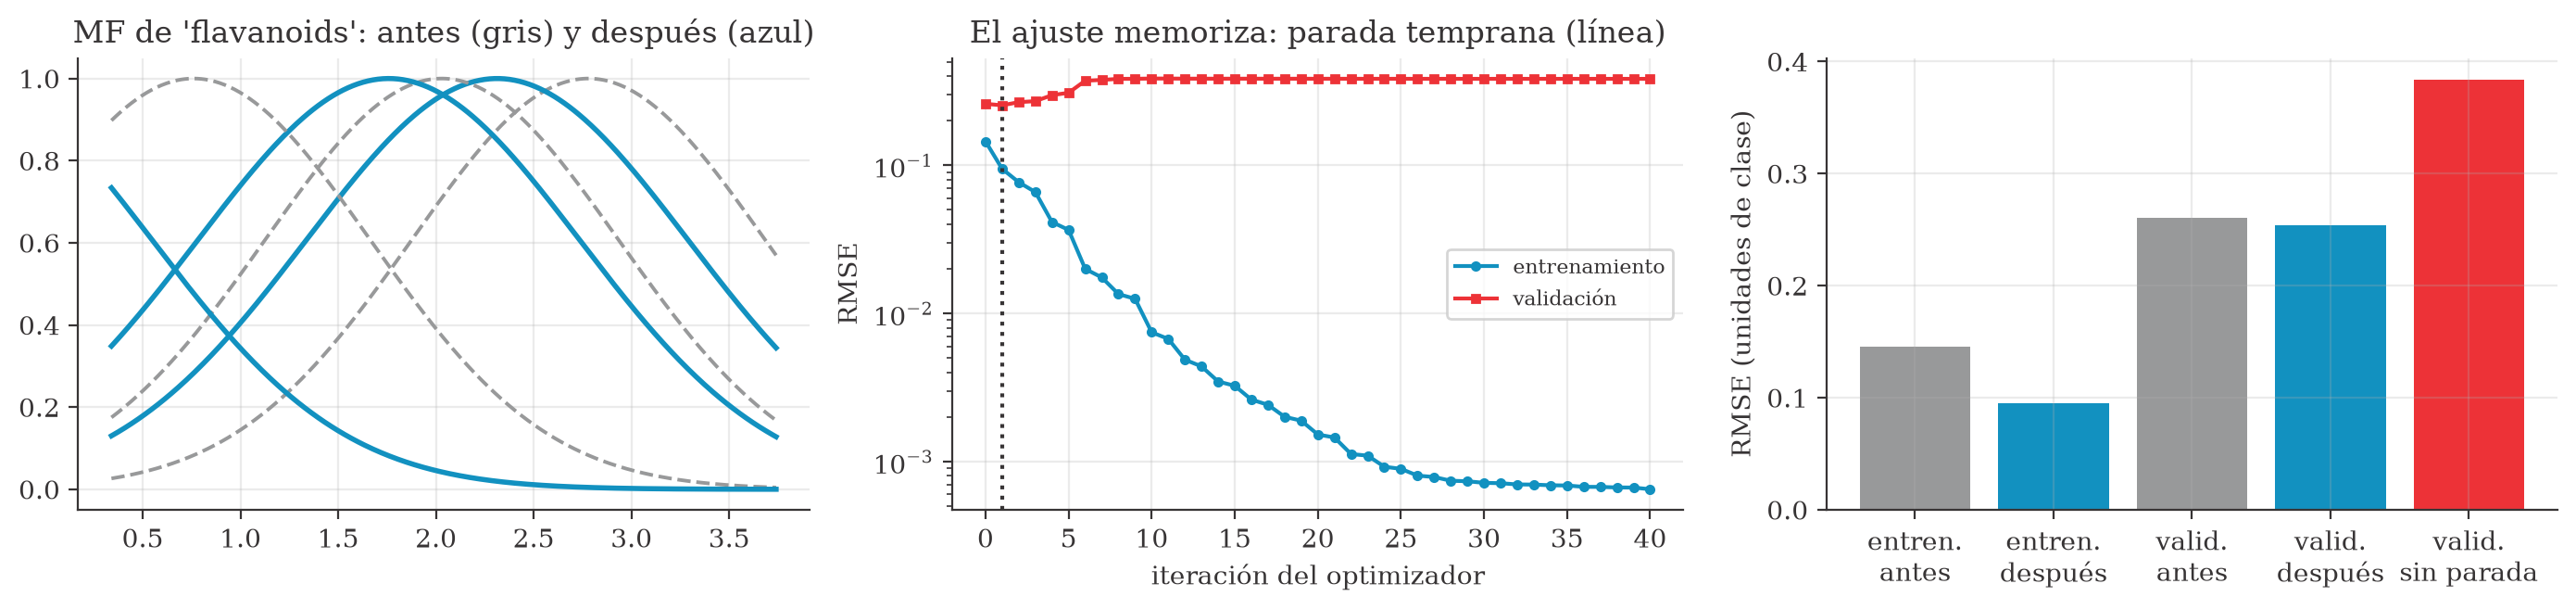
\includegraphics[width=\linewidth]{figuras/prop_f06_tune.png}\par
      \txt{Sin parada, el RMSE de validación sube \cifratuneValSubida\,\%; con parada temprana baja y la exactitud pasa de \cifratuneAccAntes{} a \cifratuneAccDesp.}
    \end{column}
    \begin{column}{0.38\textwidth}
      \UDCard{UDLightGray}{UDRed!60}{\cardtitle{UDRed}{Redondear la clase}{\fontsize{7.2pt}{8.8pt}\selectfont
        El Sugeno redondeado supone clases ordenadas. Al permutar las etiquetas de \textit{Wine}: \cifrapropPermMax{} (natural) y \cifrapropPermMin{} (otras). Wang--Mendel no cambia.\par}}
    \end{column}
  \end{columns}
\end{frame}

%% ------------------------------------------------------------------ 8
\begin{frame}{20 particiones: lo que una sola partición no dice}{Media $\pm$ desviación de la exactitud en prueba}
  \begin{columns}[T,onlytextwidth]
    \begin{column}{0.50\textwidth}
      \UDCard{white}{UDBorder}{\cardtitle{UDBlue}{Wine, 20 particiones}{\fontsize{7pt}{8.6pt}\selectfont
        \resizebox{\linewidth}{!}{\begin{tabular}{lrr}
\toprule
Método & Reglas & Exactitud en prueba \\
\midrule
Wang-Mendel n = 2 & 9,7 $\pm$ 1,2 & 0,806 $\pm$ 0,049 \\
Wang-Mendel n = 3 & 24,1 $\pm$ 3,4 & 0,865 $\pm$ 0,047 \\
Wang-Mendel n = 4 & 41,9 $\pm$ 2,9 & 0,931 $\pm$ 0,036 \\
Sustractivo r = 0,3 & 14,8 $\pm$ 2,8 & 0,881 $\pm$ 0,078 \\
Sustractivo r = 0,5 & 5,0 $\pm$ 0,9 & 0,956 $\pm$ 0,024 \\
Sustractivo r = 0,8 & 3,0 $\pm$ 0,0 & 0,946 $\pm$ 0,024 \\
Árbol de 8 hojas & 8 & 0,894 $\pm$ 0,044 \\
\bottomrule
\end{tabular}
}\par}}
    \end{column}
    \begin{column}{0.46\textwidth}
      \UDCard{UDLightGray}{UDGold}{\cardtitle{UDGold}{Lectura}{\fontsize{7.2pt}{8.8pt}\selectfont
        El sustractivo con $r=0{,}5$ a $0{,}8$ es el mejor y el más pequeño (3 a 5 reglas frente a $\approx$ 42). La diferencia entre los dos es menor que la desviación. Desviaciones de 0,03 a 0,05 son 2 o 3 vinos: una partición no basta.\par}}
    \end{column}
  \end{columns}
\end{frame}

%% ------------------------------------------------------------------ 9
\begin{frame}{Robot: qué dicen los datos}{\cifraadicN{} lecturas; 4 clases ordenadas de giro cerrado a la derecha a giro leve a la izquierda}
  \begin{columns}[T,onlytextwidth]
    \begin{column}{0.60\textwidth}
      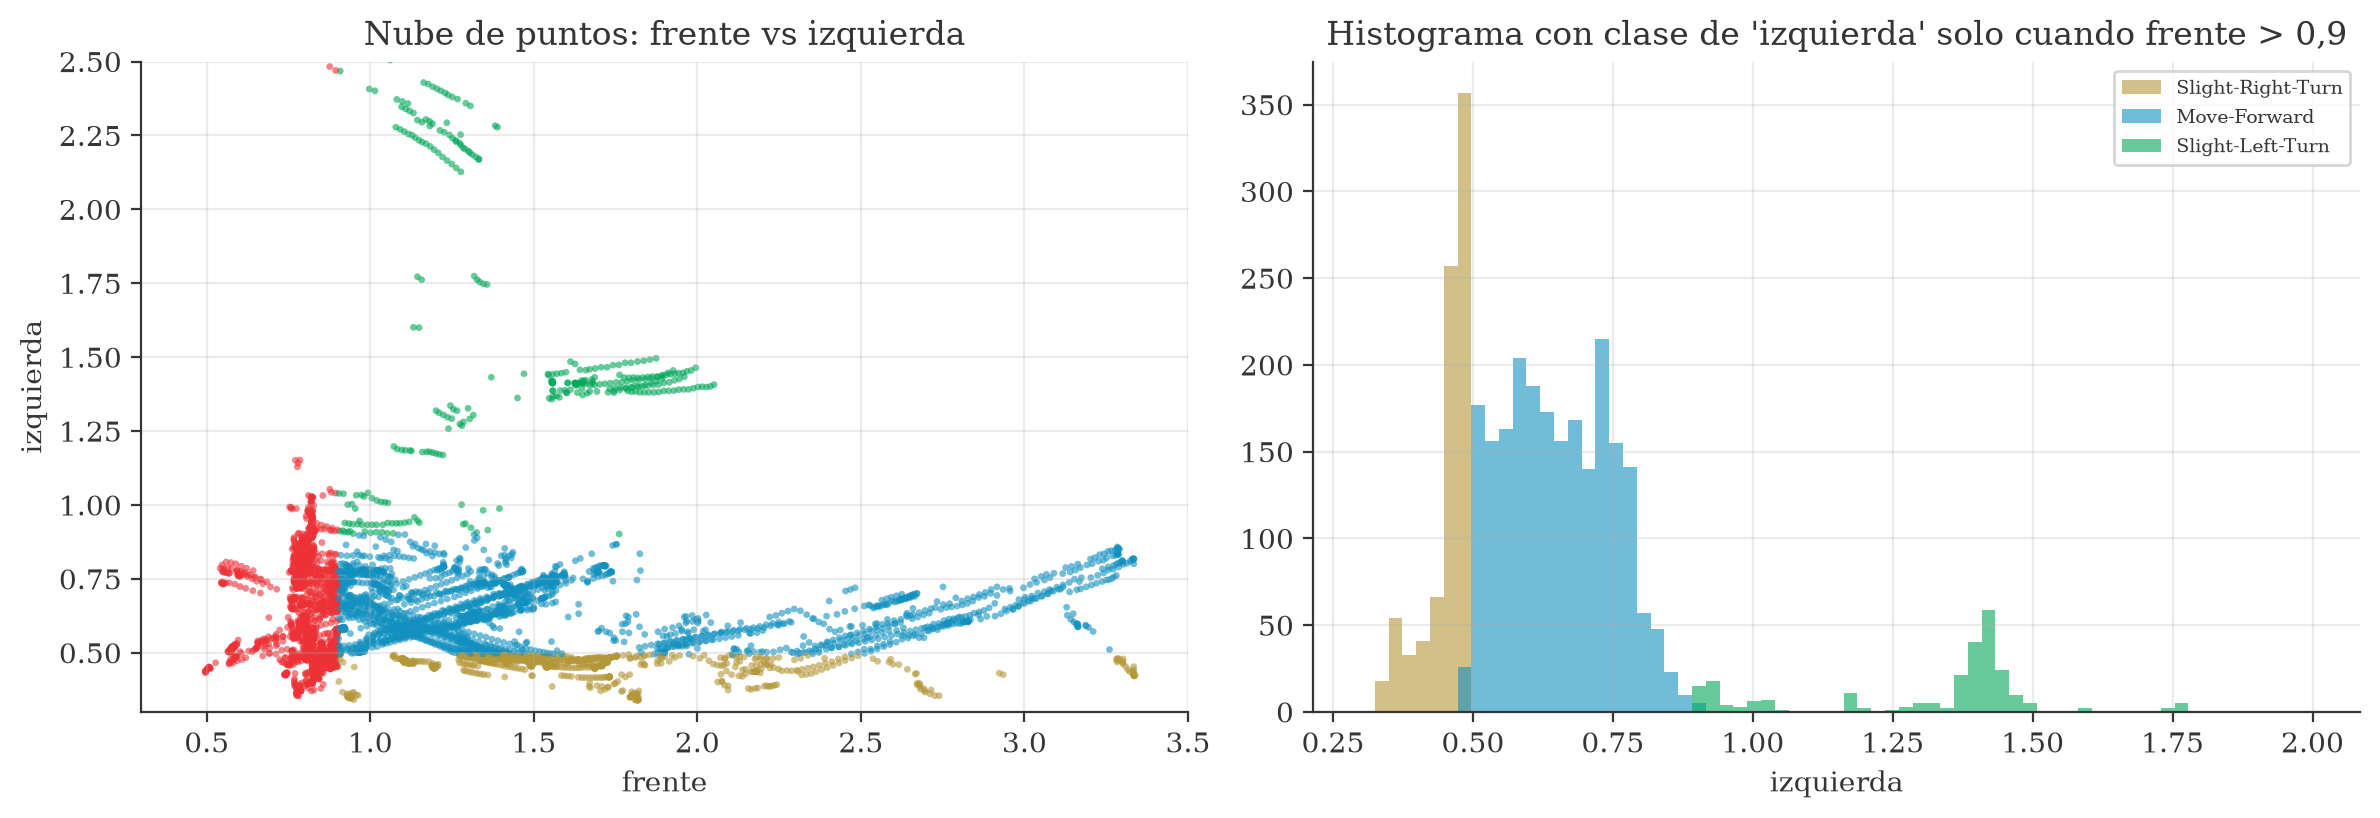
\includegraphics[width=\linewidth]{figuras/adic_f05_frente_izquierda.png}
    \end{column}
    \begin{column}{0.36\textwidth}
      \UDCard{white}{UDBorder}{\cardtitle{UDBlue}{Lo que se ve}{\fontsize{7pt}{8.6pt}\selectfont
        Las clases forman \textbf{rectángulos}: son umbrales sobre dos sensores. Frente en \cifraadicCorteFrente; izquierda en \cifraadicCorteIzqA{} y \cifraadicCorteIzqB. Derecha y atrás no aportan.\par}}
      \vspace{0.1cm}
      \txt{Es una serie en el tiempo (racha típica de \cifraadicRacha{} lecturas): se prueba con bloques de 100.}
    \end{column}
  \end{columns}
\end{frame}

%% ------------------------------------------------------------------ 10
\begin{frame}{Robot: funciones de pertenencia y modelos}{Los cruces van donde cambia la clase; $w$ = ancho de la zona difusa}
  \begin{center}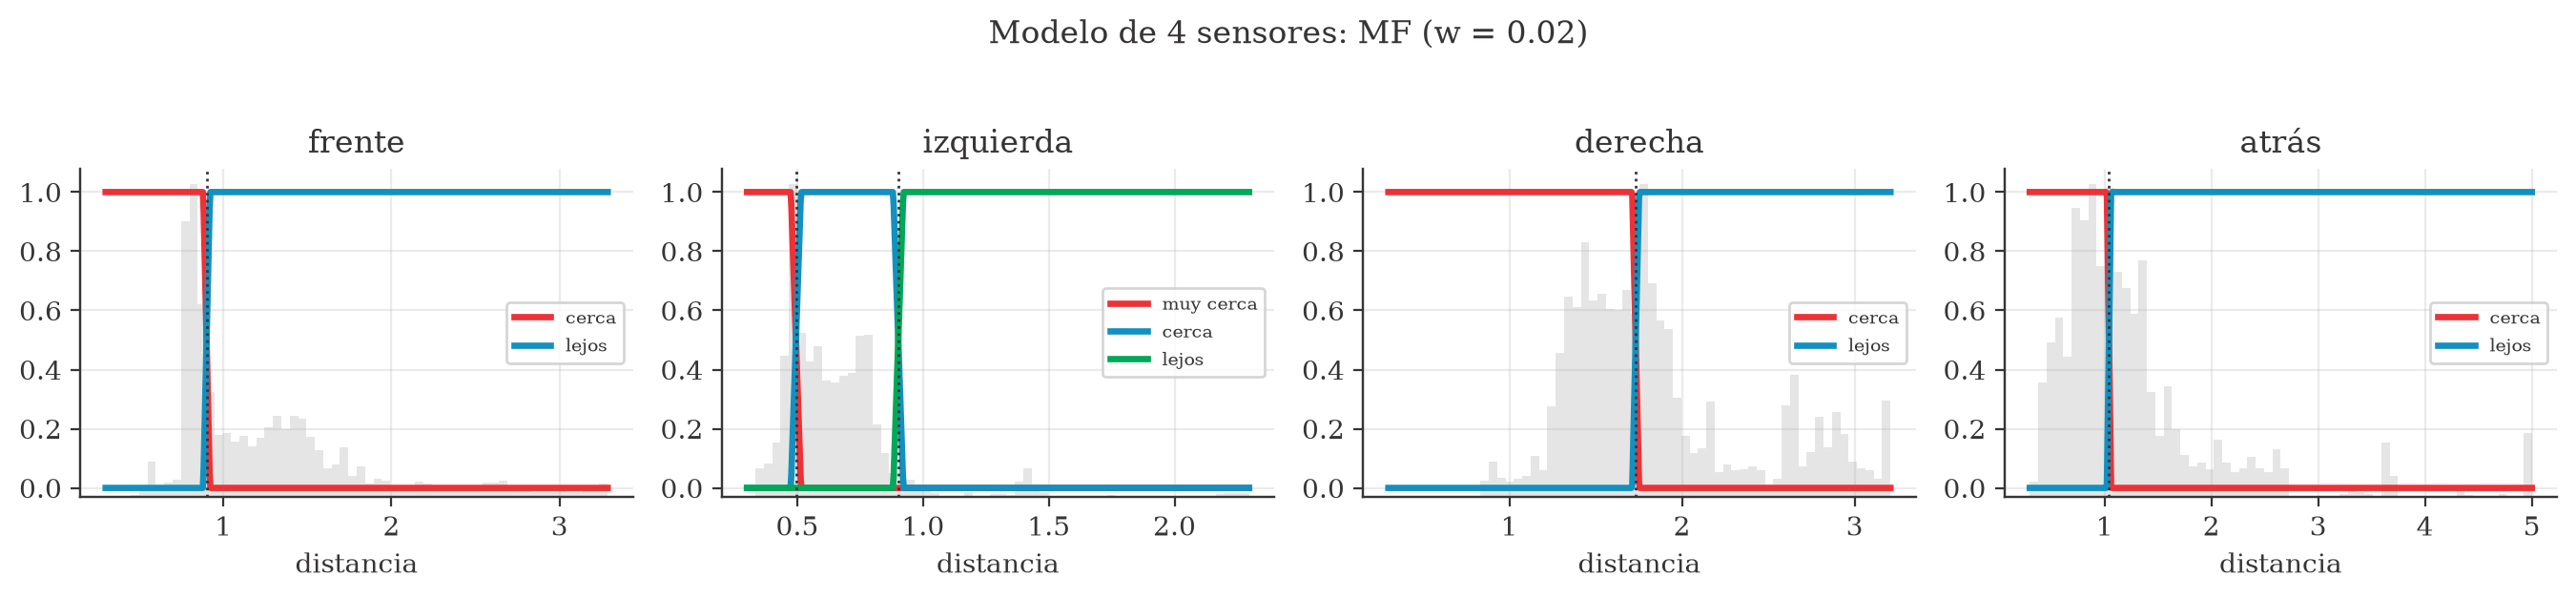
\includegraphics[width=0.93\linewidth]{figuras/adic_f07_mf_4sensores.png}\end{center}
  \vspace{-0.1cm}
  \begin{columns}[T,onlytextwidth]
    \begin{column}{0.48\textwidth}
      \UDCard{white}{UDBorder}{\cardtitle{UDBlue}{2 sensores}{\fontsize{7.2pt}{8.8pt}\selectfont
        $2\times3=$ \textbf{\cifraadicDosReglas{} reglas}; exactitud \textbf{\cifraadicDosAcc\,\%}, balanceada \cifraadicDosBal\,\%.\par}}
    \end{column}
    \begin{column}{0.48\textwidth}
      \UDCard{UDLightGray}{UDRed!60}{\cardtitle{UDRed}{4 sensores}{\fontsize{7.2pt}{8.8pt}\selectfont
        $2\times3\times2\times2=$ \textbf{\cifraadicCuatroReglas{} reglas}; exactitud \textbf{\cifraadicCuatroAcc\,\%}, balanceada \cifraadicCuatroBal\,\%.\par}}
    \end{column}
  \end{columns}
\end{frame}

%% ------------------------------------------------------------------ 11
\begin{frame}{Robot: el análisis importa, y también cómo se evalúa}{Mismo límite de 100 reglas}
  \begin{columns}[T,onlytextwidth]
    \begin{column}{0.58\textwidth}
      \UDCard{white}{UDBorder}{\cardtitle{UDBlue}{Diseños de MF}{\fontsize{6.2pt}{7.6pt}\selectfont
        \resizebox{\linewidth}{!}{\begin{tabular}{llrrrrr}
\toprule
Modelo & Diseño de las MF & MF & Reglas & CV & Exactitud & Exact. bal. \\
\midrule
2 sensores & uniforme (auto.) & 6-10 & 60 & 95,4\,\% & 91,4\,\% & 94,2\,\% \\
2 sensores & cuantiles (auto.) & 6-8 & 48 & 96,7\,\% & 94,4\,\% & 96,3\,\% \\
2 sensores & fcm (auto.) & 8-10 & 80 & 95,6\,\% & 96,1\,\% & 97,3\,\% \\
2 sensores & cortes del análisis & 2-3 & 6 & 99,8\,\% & 99,8\,\% & 99,9\,\% \\
4 sensores & uniforme (auto.) & 5-5-2-2 & 100 & 86,7\,\% & 78,7\,\% & 80,8\,\% \\
4 sensores & cuantiles (auto.) & 3-4-3-2 & 72 & 95,4\,\% & 95,2\,\% & 96,3\,\% \\
4 sensores & fcm (auto.) & 5-5-2-2 & 100 & 90,0\,\% & 83,6\,\% & 83,0\,\% \\
4 sensores & cortes del análisis & 2-3-2-2 & 24 & 99,8\,\% & 99,5\,\% & 99,4\,\% \\
\bottomrule
\end{tabular}
}\par}}
    \end{column}
    \begin{column}{0.38\textwidth}
      \UDCard{UDLightGray}{UDGold}{\cardtitle{UDGold}{Dos lecciones}{\fontsize{7pt}{8.6pt}\selectfont
        \textbf{Más reglas $\neq$ mejor:} los diseños automáticos rinden de \cifraadicAutoCuatroMin{} a \cifraadicAutoDosMax.\\[2pt]
        \textbf{Series de tiempo:} con lecturas sueltas, kNN pasa de \cifraadicKnnBloques{} a \cifraadicKnnMuestra{} (+\cifraadicKnnInfla\pts{} de fuga).\par}}
    \end{column}
  \end{columns}
\end{frame}

%% ------------------------------------------------------------------ 12
\begin{frame}{Conclusiones}{Lo que funcionó y lo que hay que saber}
  \begin{columns}[T,onlytextwidth]
    \begin{column}{0.48\textwidth}
      \UDCard{white}{UDBorder}{\cardtitle{UDBlue}{Lo que funcionó}{\fontsize{7.3pt}{9pt}\selectfont
        \begin{itemize}\setlength{\itemsep}{1pt}
          \item Reproducir el script: 9 de 9 referencias.
          \item Sustractivo ($r=0{,}5$ a $0{,}8$): 3 a 5 reglas y $\approx$ 95\,\%.
          \item Robot: \cifraadicDosReglas{} y \cifraadicCuatroReglas{} reglas con $>99$\,\%.
        \end{itemize}\par}}
    \end{column}
    \begin{column}{0.48\textwidth}
      \UDCard{UDLightGray}{UDRed!60}{\cardtitle{UDRed}{Lo que hay que saber}{\fontsize{7.3pt}{9pt}\selectfont
        \begin{itemize}\setlength{\itemsep}{1pt}
          \item $r$ pequeño sobreajusta; validar cruzado.
          \item Ajustar sin validación memoriza.
          \item Redondear clases supone un orden.
          \item Series de tiempo: evaluar por bloques.
        \end{itemize}\par}}
    \end{column}
  \end{columns}
  \vspace{0.15cm}
  \txt{\textbf{Límites:} no se ejecutó MATLAB (se reprodujeron sus vistas y su idea en Python); una partición 70/30 en Wine; nombres de sensores tomados del conjunto original.}
\end{frame}

\UDcierre{Juan Felipe Rodríguez Galindo}
         {Maestría en Ciencias de la Información\\y las Comunicaciones}
         {Inteligencia Computacional Aplicada}

\end{document}
